\label{inversion_case_study}
The following case study illustrates how the \code{inversion} and \code{grabsample} subcommands 
can be used in tandem to perform multiple cycles of source inversion calculations as more and more measurement data becomes available. 
The solution approach integrates iterative sampling strategy for finding the contamination source using discrete measurements 
obtained from manual grab samples taken during different sampling cycles.  
Figure \ref{fig:inversion_flowchart} illustrates the source inversion and grab sample strategy. 
A contamination incident is first suspected given a customer inquiry or detection from a fixed continuous 
sensor in the Contamination Warning System (CWS). 
At this stage, a team is sent out to gather manual grab samples at and around the location of first detection. 
Discrete yes/no measurements from these manual grab samples along with the measurement from CWS 
are then used to identify the potential sources of the contamination incident.
Since the inversion problem is an ill-posed problem, the solution will generally be non-unique. 
A set of likely locations can be identified and the \code{grabsample} subcommand can be used 
to determine the location of the next manual grab samples. The source inversion is performed again using the new information. 
This cycle of collecting manual grab samples and performing source inversion is continued until the true injection location(s) is identified. 
\begin{figure}[!ht]
\begin{center}
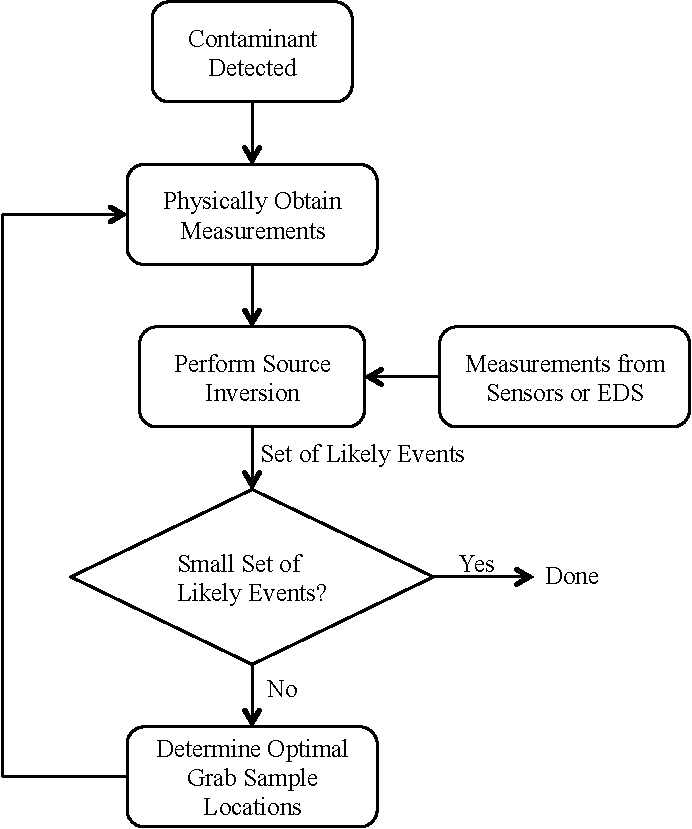
\includegraphics[scale=0.6]{graphics/inversion_strategy.pdf}
\caption{Illustration of the source inversion and grab sample cycling strategy.}
\label{fig:inversion_flowchart}
\end{center}
\end{figure}

\subsection{Case Study}
Since real system data is not available, the \code{measuregen}
executable is used to generate simulated data for the contamination incident in the following case study.  In this simulation, 
a conservative contaminant is injected into node 163 of EPANET
Example Network 3 (Net3) starting at 8 AM.  The Bayesian probability
based formulation [\ref{sec.bayesian_algorithm}] is used in
the \code{inversion} subcommand to identify the possible contamination
sources. Figure \ref{fig:case_study_setup} shows the fixed sensor
locations in blue while the original contamination location is shown
in red.  The CWS consists of five fixed sensors that provide
measurements every 15 minutes (set as a command line option in \code{measuregen}).

\begin{figure}[ht!]
\begin{center}
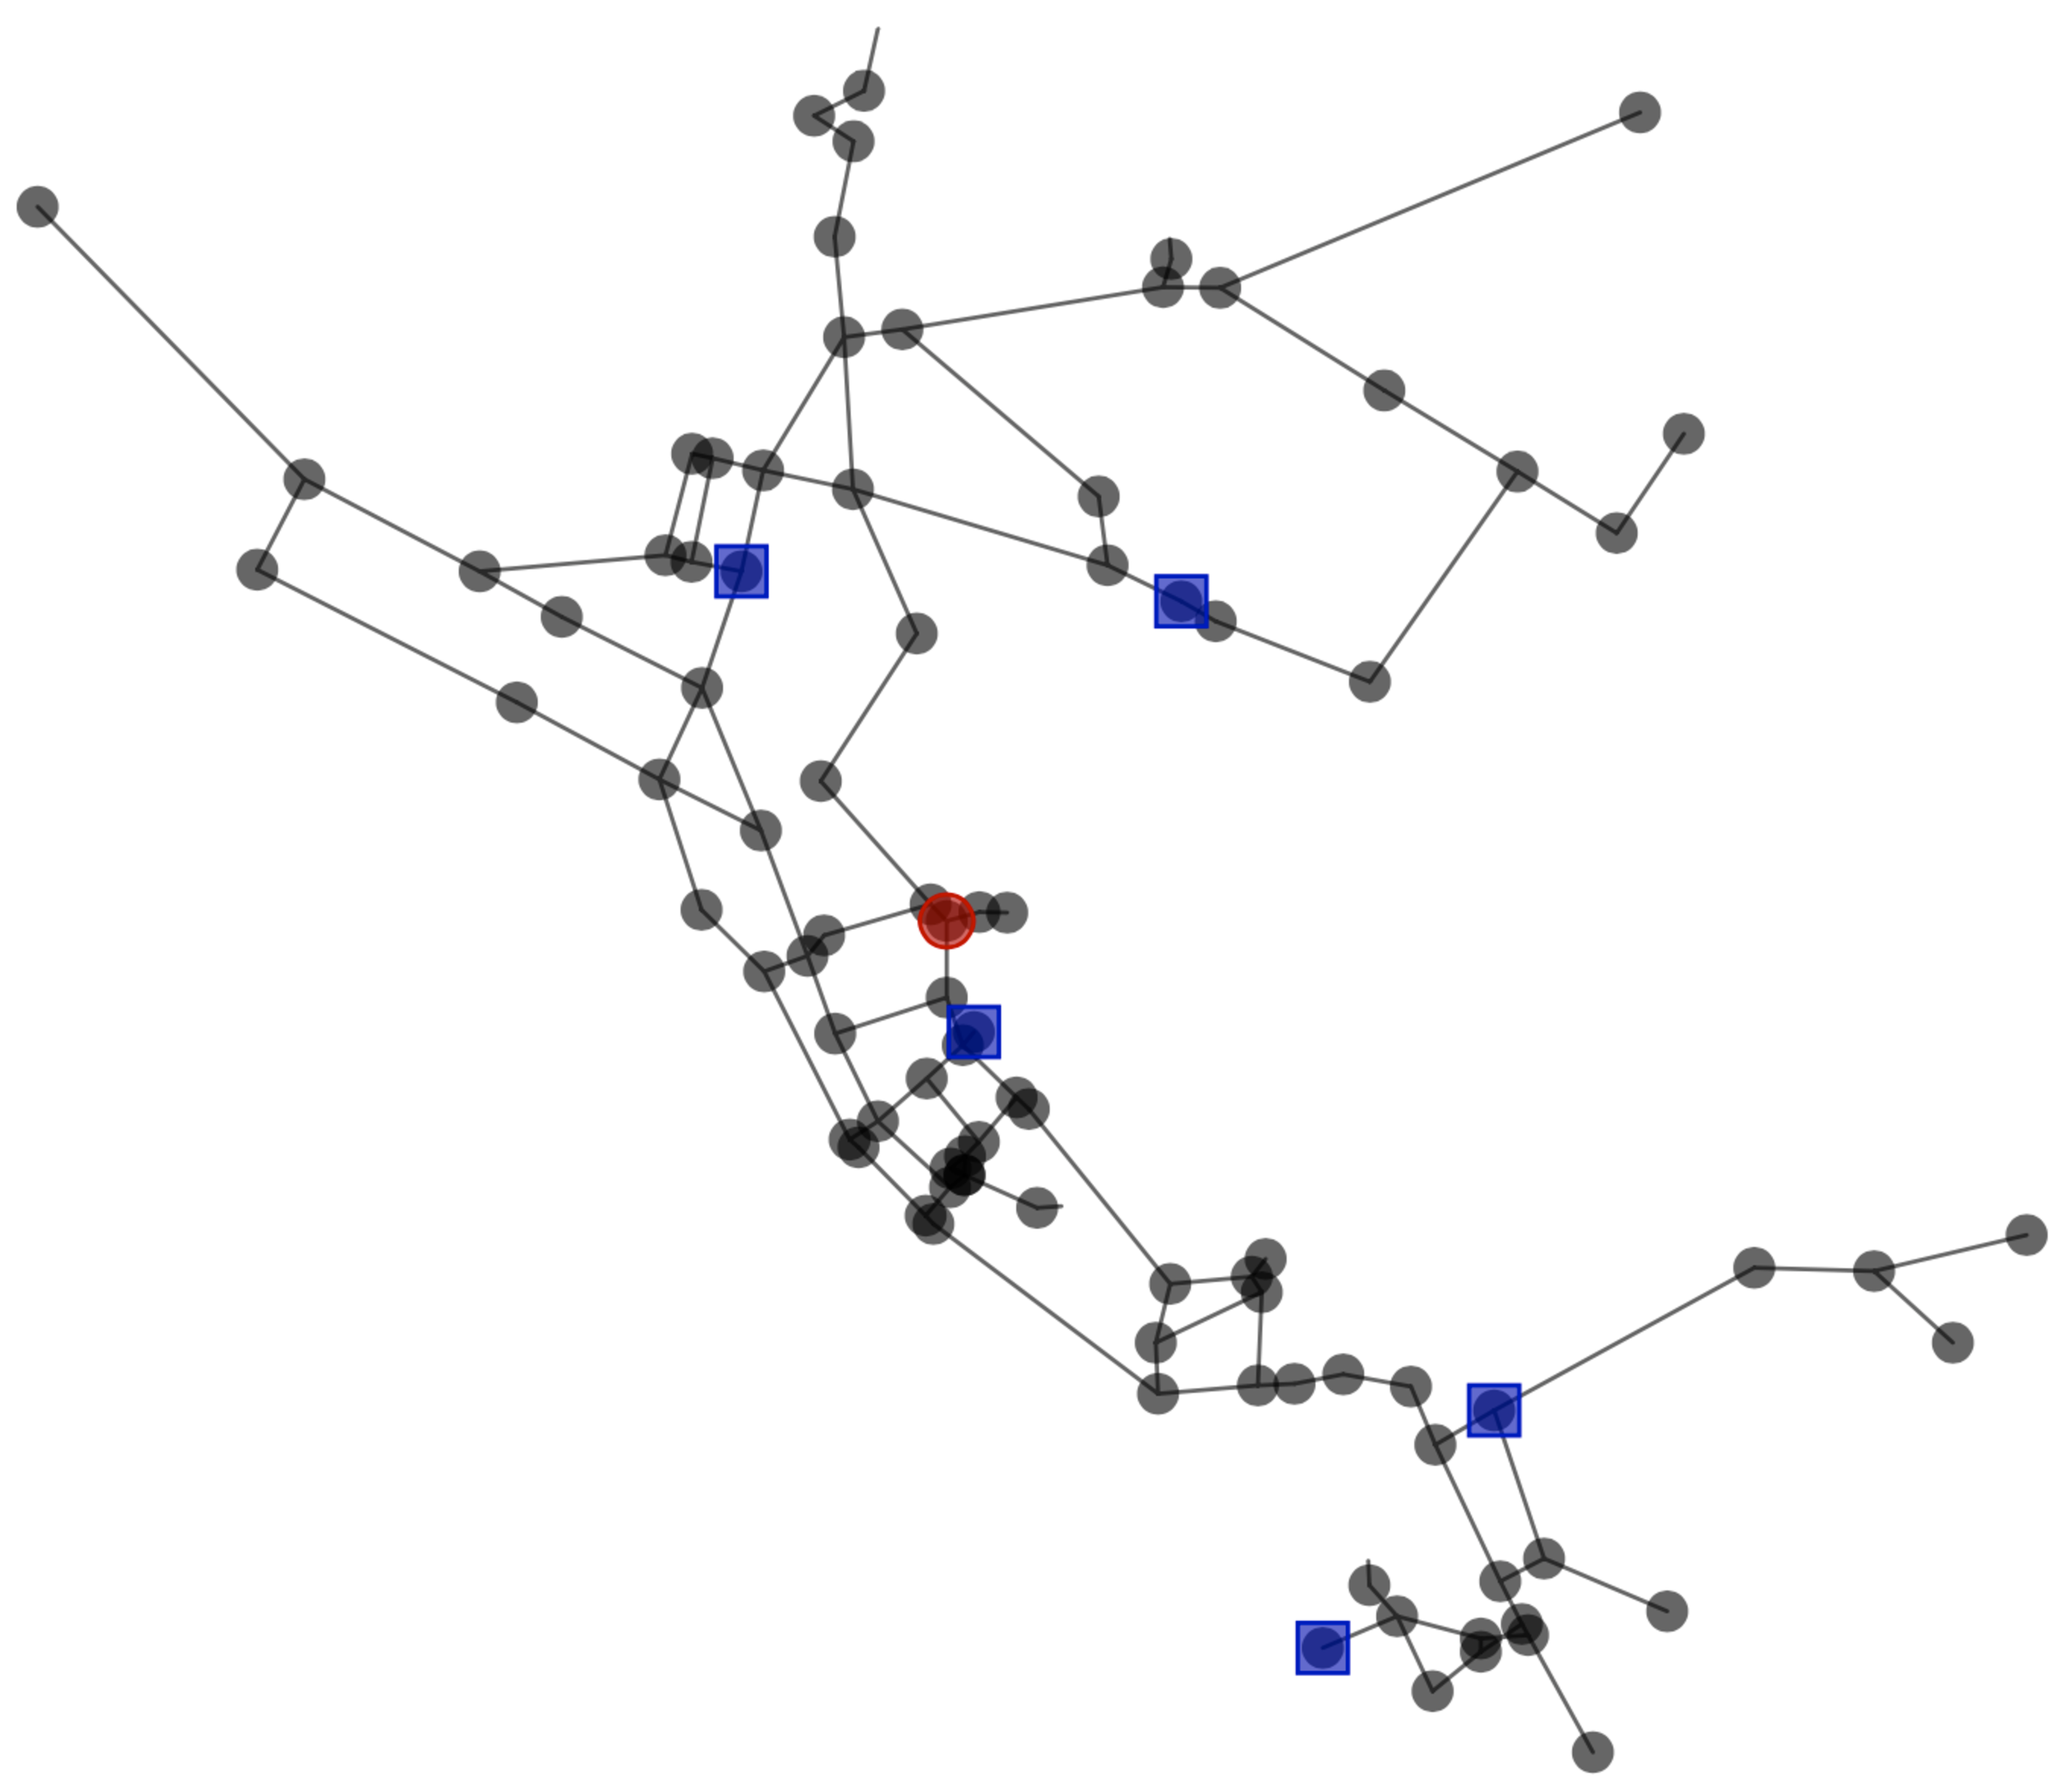
\includegraphics[scale=0.25]{graphics/inversion_cs_setup.pdf}
\caption{Fixed sensors (blue) and contamination location (red) for case study.}
\label{fig:case_study_setup}
\end{center}
\end{figure}

All the files required for this case study are provided in the \code{examples/case\_studies/inversion} folder.
  
The case study is a composed of three cycles of source inversion and grab sampling to reduce the number of possible contamination source 
locations. During each cycle, the \code{inversion} subcommand uses the following data:
\begin{itemize}
\item Net3.inp - EPANET Example Network 3 input (INP) file.
\item MEASURES.dat - Measurements file binary (yes/no) results from fixed sensors and grab samples (generated using \code{measuregen} executable).
\item \textit{<output\_prefix>}\_Likely\_Nodes.dat - Likely nodes file containing a list of feasible nodes to consider as possible contamination source nodes. 
This file is only used in cycles 2 \& 3. 
\end{itemize}      
The \code{inversion} subcommand outputs a YAML file with a list of possible contamination sources. 
A TSG file is also created that provides information about the possible contamination incidents. This file 
can be used in the \code{grabsample} subcommand. Thereafter, Cycles 1 \& 2 use the following data to determine optimal sample location:

\begin{itemize}
\item Net3.inp - EPANET Example Network 3 input (INP) file.
\item \textit{<output\_prefix>}\_profile.tsg - TSG file which contains a list of likely injections obtained 
from the \code{inversion} subcommand from the preceding cycle.
\item Sample time - Time in the future when the samples are expected to be taken. This is generally the current time 
plus the time it would take the sample teams to obtain measurements. 
\item fixed\_sensors.dat - List of fixed continuous sensor locations. This is used to avoid fixed sensors being selected
as grab sample locations.  

\end{itemize}

\subsection{Cycle 1}
At 8:15 AM, the sensor located at node 167 detects abnormal water quality. Further confirmation is made with another positive 
measurement at 8:30 AM. At this point, the measurement data from the past 8 hours is used to perform source inversion. 
The \code{inversion} subcommand identifies 24 possible injection locations as shown in red 
in Figure \ref{fig:case_study_cycle1}. The \code{grabsample} subcommand is then used to identify additional measurement 
locations that will reduce the number of possible injection locations. 
The utility has three teams available to gather manual grab samples and it takes 30 minutes for each team to 
obtain the manual samples. The \code{grabsample} subcommand identifies the three optimal grab sample locations 
shown in blue and the possible injection nodes in red in Figure \ref{fig:case_study_cycle1}.             

\begin{figure}[!ht]
\begin{center}
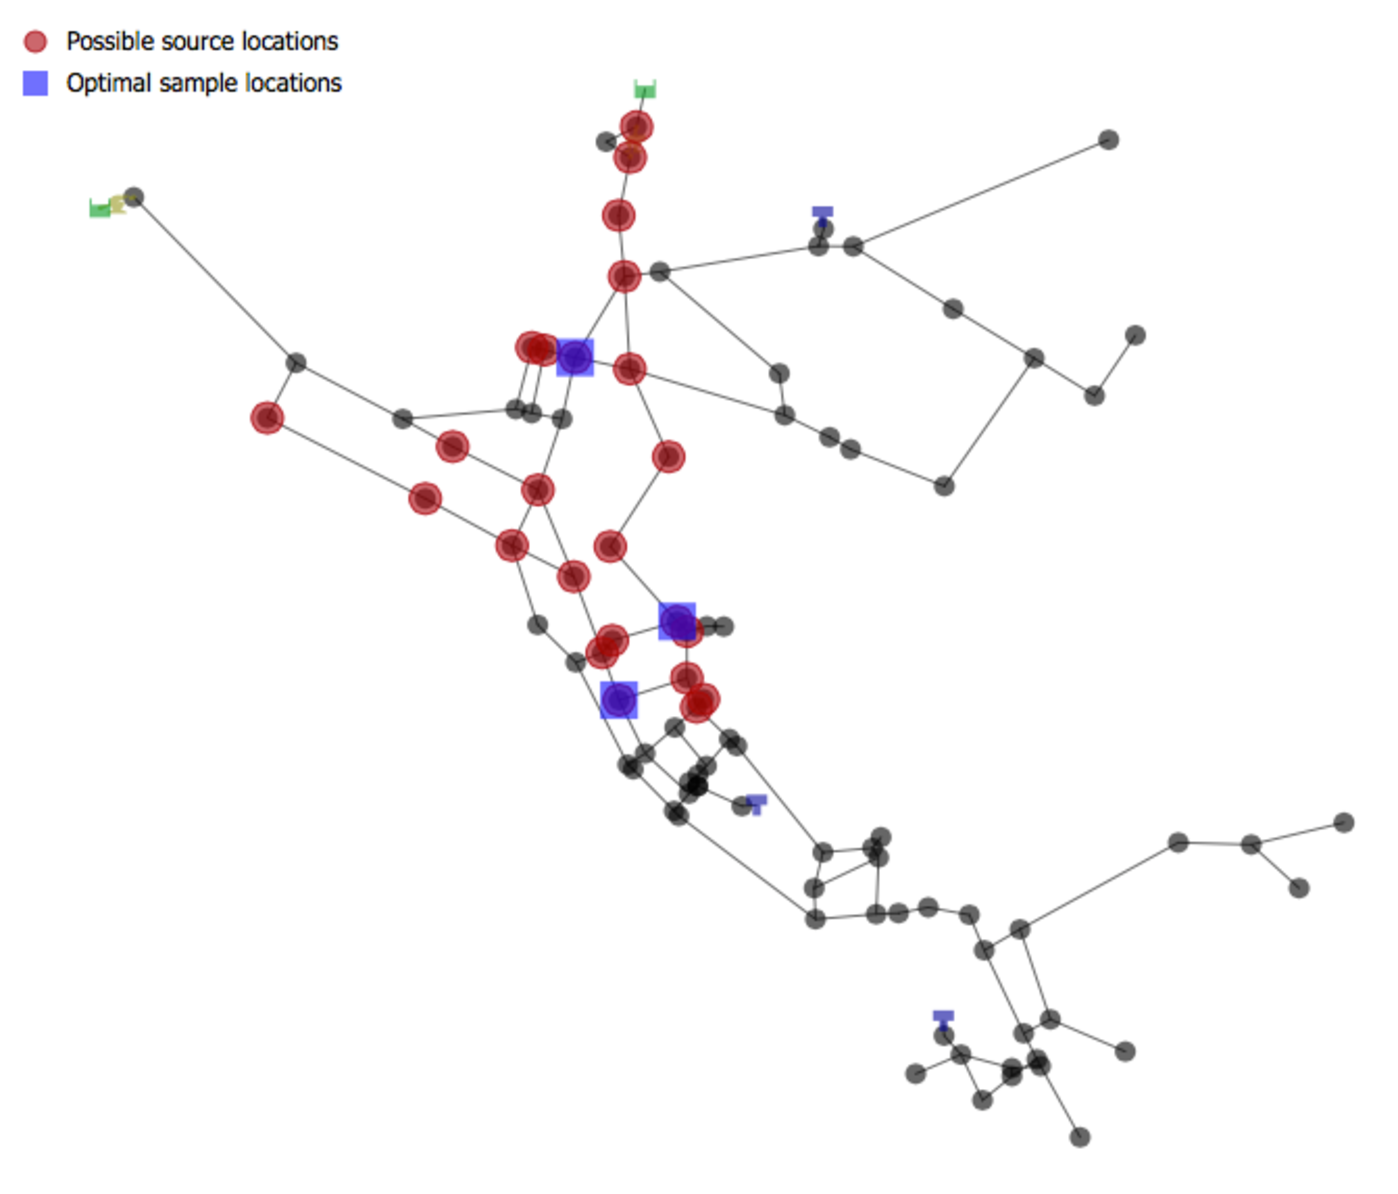
\includegraphics[scale=0.6]{graphics/inversion_cs_cycle1.pdf}
\caption{Cycle 1 identified optimal grab sample locations (blue).}
\label{fig:case_study_cycle1}
\end{center}
\end{figure}

The files required and generated during this cycle of source inversion and grab sample 
are provided in the \code{examples/case\_studies/inversion/Cycle1} folder. 

\subsection{Cycle 2}
In the 30 minutes that the sampling teams take to get manual grab sample measurements from the locations identified in Cycle 1, 
new measurements are also available from the fixed sensors in the CWS. It is assumed that
the sampling teams have field instruments that can provide them with a yes/no indication of the
presence or absence of a contaminant.  
At 9:00 AM, these new measurements are used to perform source inversion again. 
This time the \code{inversion} subcommand identifies seven possible injection locations as shown in Figure \ref{fig:case_study_cycle2}. 
In Cycle 2, the possible sources were restricted to the 24 nodes identified in Cycle 1 using the feasible nodes option. 
Again a 30-minute delay for sample collection and three sample teams were used in the \code{grabsample} subcommand to identify 
the optimal grab sample locations at 9:30 AM. These grab sample locations (blue) and 
the possible injection nodes (red) are shown in Figure \ref{fig:case_study_cycle2}.

\begin{figure}[!ht]
\begin{center}
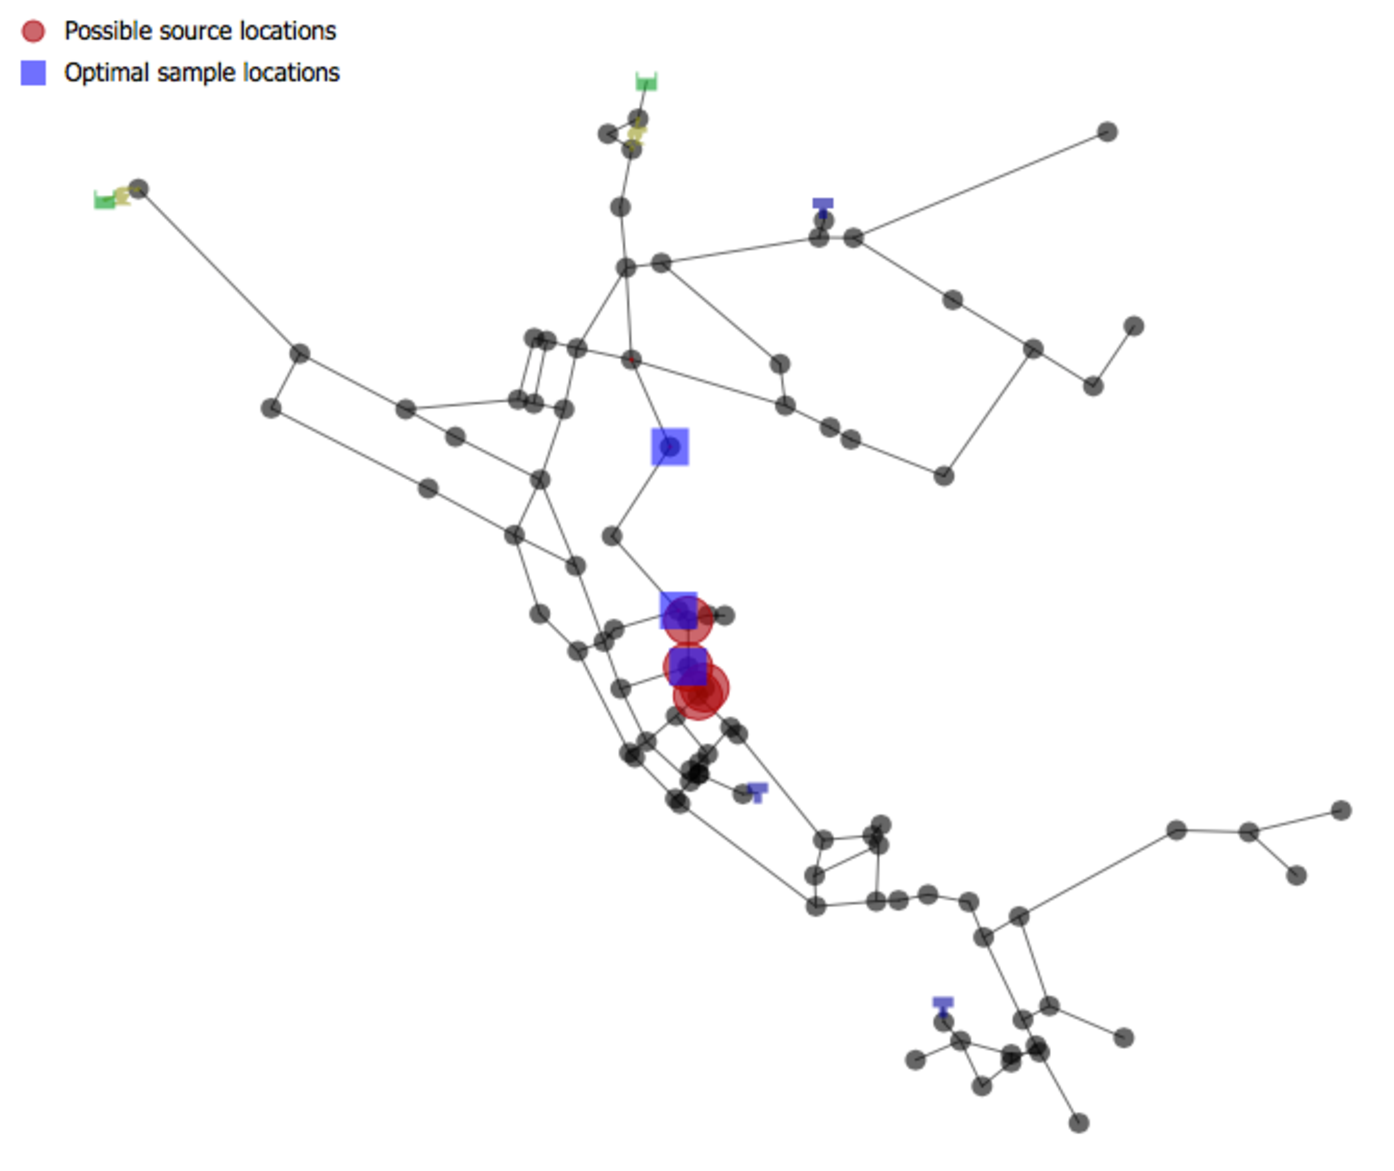
\includegraphics[scale=0.6]{graphics/inversion_cs_cycle2.pdf}
\caption{Cycle 2 identified optimal grab sample locations (blue).}
\label{fig:case_study_cycle2}
\end{center}
\end{figure}

The files required and generated during this cycle of source inversion and grab sample are 
provided in the \code{examples/case\_studies/inversion/Cycle2} folder.  
        
\subsection{Cycle 3}
Grab sample measurements are obtained at 9:30 AM from the optimal locations identified in Cycle 2. 
These along with the new measurements obtained from the fixed sensors are used to perform source inversion again. 
Only the seven possible injection nodes obtained in Cycle 2 are considered as feasible nodes in the \code{inversion} subcommand 
for Cycle 3. Three possible injection locations as shown in Figure \ref{fig:case_study_cycle3} are identified in this cycle.

\begin{figure}[!ht]
\begin{center}
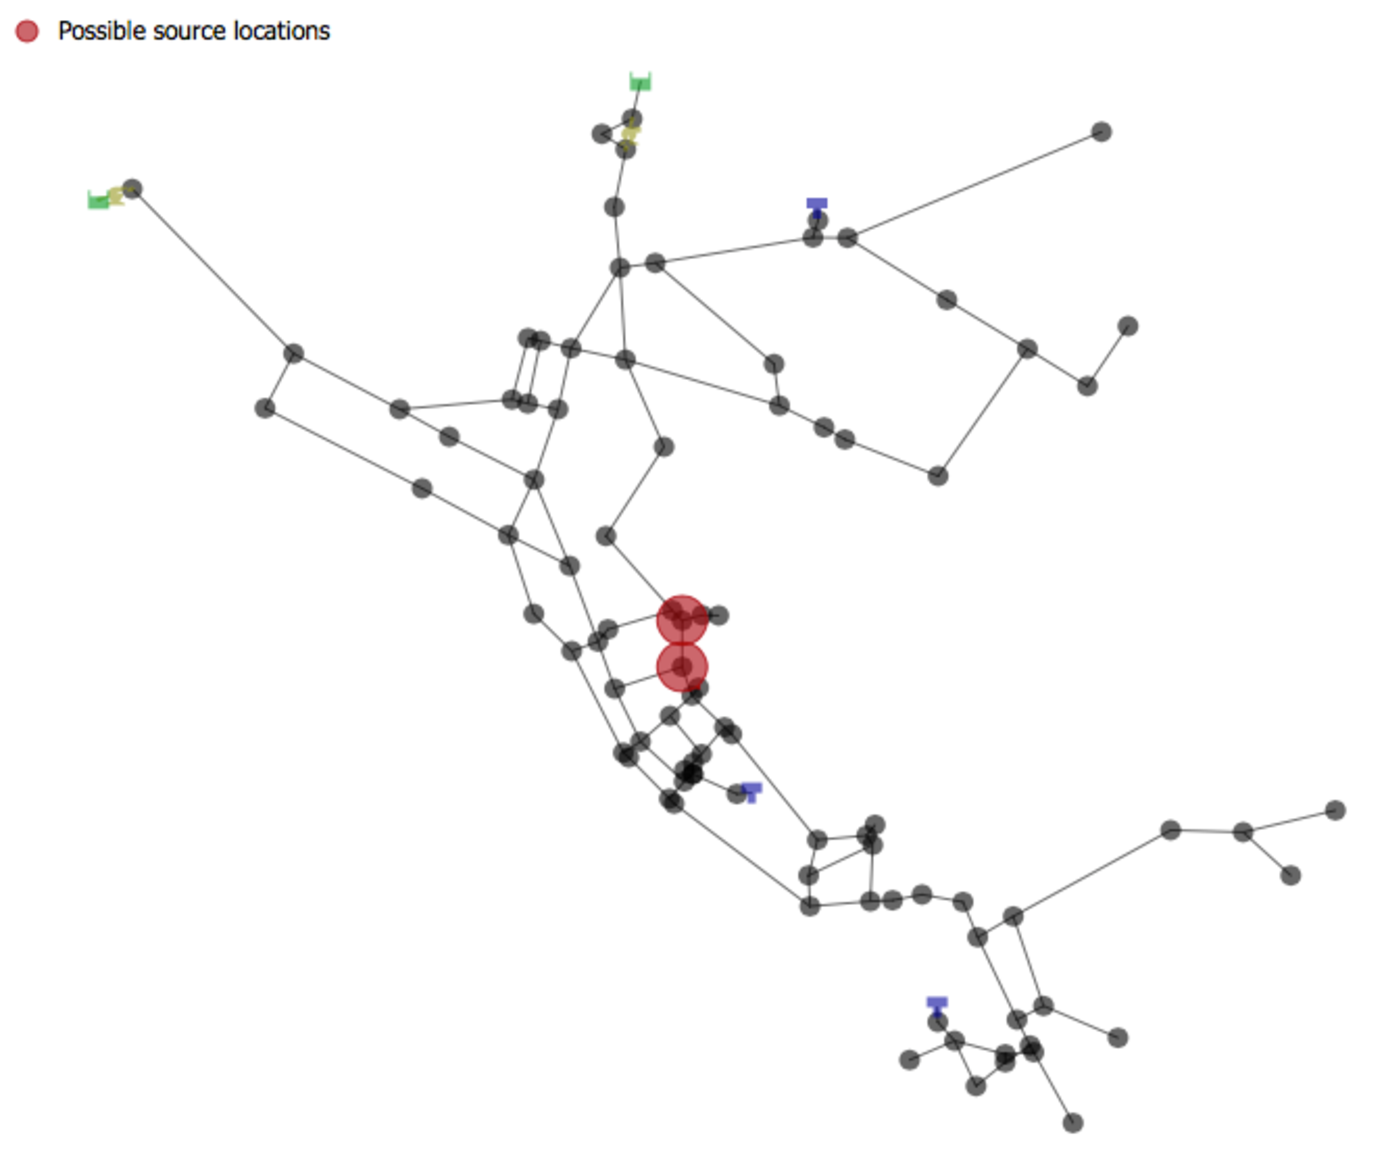
\includegraphics[scale=0.6]{graphics/inversion_cs_cycle3.pdf}
\caption{The possible injection nodes (red) identified in Cycle 3.}
\label{fig:case_study_cycle3}
\end{center}
\end{figure}

Since the water utility has three sampling teams available, the teams can directly inspect the three possible injection locations 
identified in this cycle to confirm the true injection location.  
